%!TEX root = index.tex
\chapter{Testes e Resultados}
\label{cha:testes_e_resultados}
Conforme introduzido anteriormente o produto da empresa Beeconnect é o aplicativo com o mesmo o nome. Tal produto foi desenvolvido para as plataformas Android e iOS e consiste basicamente em um aplicativo para descontos em lojas físicas. O seu principal diferencial é a geolocalização indoor precisa com uso de um aparelho chamado beacon. Quando um usuário do aplicativo passar por um beacon localizado dentro de uma loja parceira ele pode receber uma notificação informando que ele recebeu um desconto especial em um produto relevante ou receber um simples "Bem vindo" conforme mostrado na \autoref{fig:bemvindo_beeconnect}.

\begin{figure}[H]
\caption{Exemplo de notificação do aplicativo Beeconnect}
\centerline{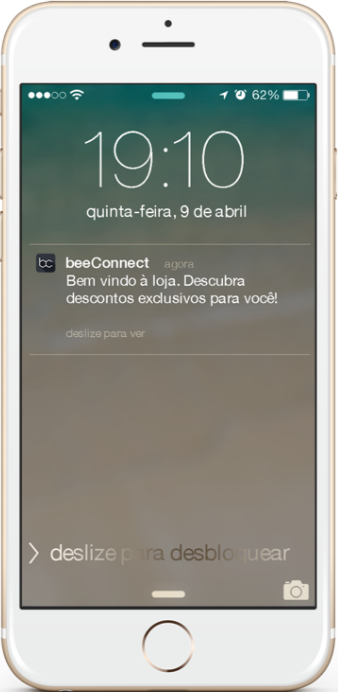
\includegraphics[scale=0.35]{img/bemvindo_beeconnect}}
\label{fig:bemvindo_beeconnect}
\caption* {Fonte: https://app.beeconnect.com.br/}
\end{figure}

Até o momento em que os testes foram realizados a Beeconnect contava com cerca de 2000 downloads do aplicativo, 1600 usuários cadastrados e 10 empresas parceiras. Um dos problemas é que nenhuma loja ainda estava disposta a pagar pela plataforma.

Os principais desafios da Beeconnect são:
\begin{itemize}
\item Crescer a base de lojas pagantes dentro do aplicativo.
\item Crescer a base de usuários de forma barata.
\end{itemize}

Como mencionado previamente tais desafios eram realmente difíceis porque muitos usuários só baixariam o aplicativo se ele possuísse mais lojas participantes, assim como muitas lojas só se interessavam pela base de usuários e só entrariam no aplicativo caso a base fosse grande, com mais de cem mil usuários.

Baseando-se na metodologia apresentada no capítulo anterior o autor então começou a desenvolver os testes e resultados que serão apresentados nesse capítulo. Foram feitas duas iterações no ciclo explicitado pela metodologia introduzida no capítulo anteriror.

\section{Mapear estado atual da startup}
\label{cha:mapear_estado}
O autor elaborou um canvas inicial, ilustrado na \autoref{fig:canvas_beeconnect_1}, baseado nas premissas iniciais da empresa: 

\begin{figure}[H]
\caption{Canvas de Modelo de Negócio inicial da Beeconnect}
\centerline{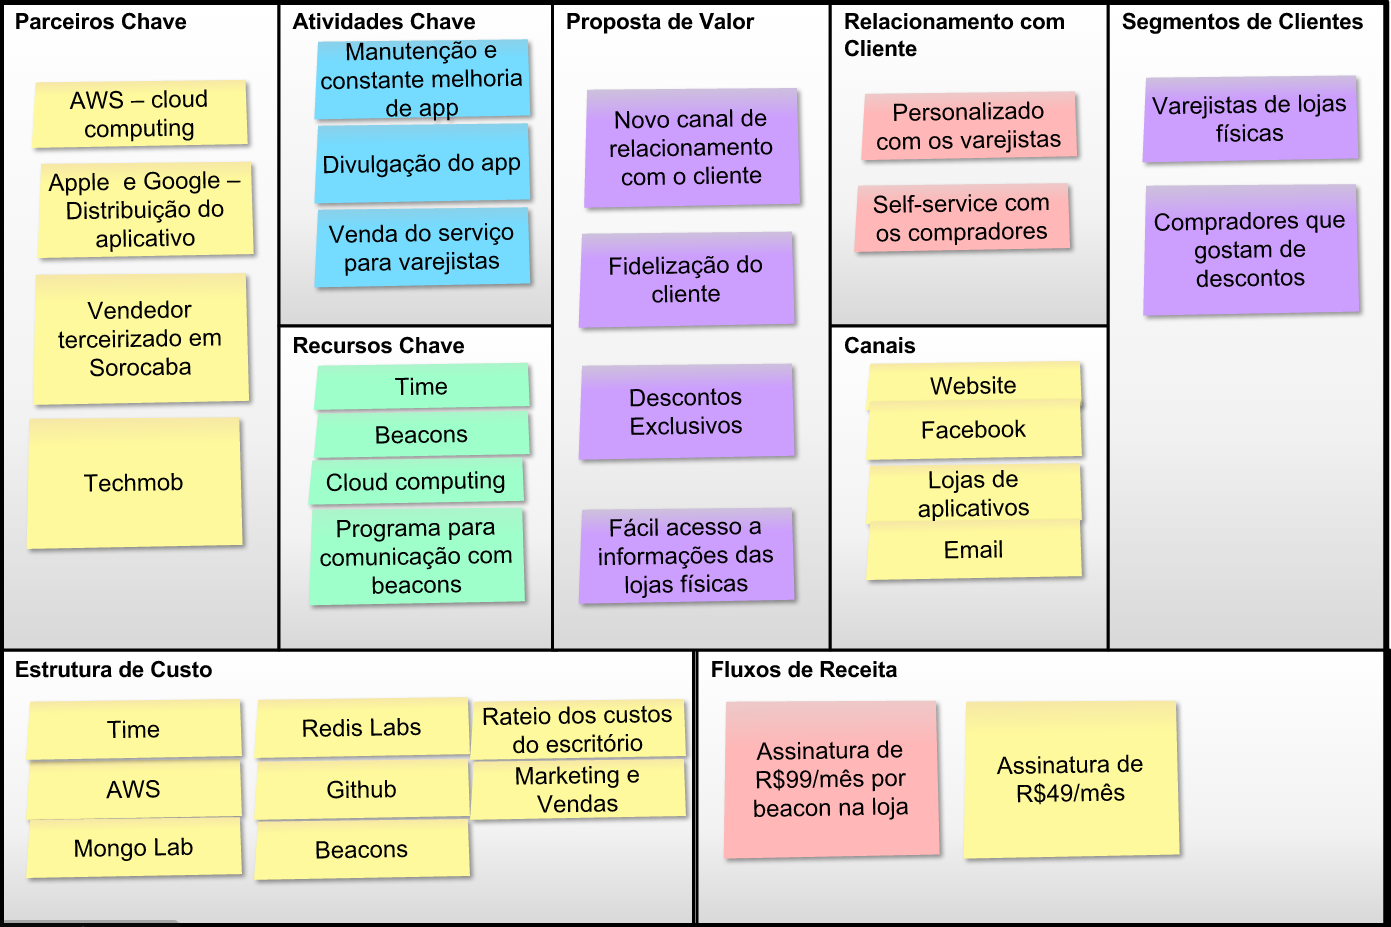
\includegraphics[scale=0.25]{img/canvas_beeconnect_1}}
\label{fig:canvas_beeconnect_1}
\caption* {Fonte: Elaborado pelo autor}
\end{figure}

Foram detalhados então cada um dos nove blocos do Canvas de Modelo de Negócio.
\subsection{Segmentos de Clientes}
\label{cha:segmentos_de_clientes}
Os segmentos de clientes para o aplicativo são:
\begin{itemize}
\item Varejistas de lojas físicas, que serão tratados daqui em diante como "Lojas": 
\item Frequentadores de lojas físicas que gostam de descontos, que serão tratados aqui em diante como "Usuários": 
\end{itemize}
Deste modo verificou-se que o produto atende dois segmentos distintos porém dependentes, típico de um mercado Multilateral. Por exemplo: sem uma boa diversidade de Lojas dentro do aplicativo não há muitas opções de descontos para os Usuários.

\subsection{Proposição de Valor}
\label{cha:proposicao_de_valor}
Dado que o produto atende um segmento multilateral de clientes ele tem que gerar valor para ambos os segmentos.
\begin{itemize}
\item Novo canal de relacionamento com o cliente: os lojas físicas tem no aplicativo uma nova plataforma para se comunicar com seus clientes. Elas podem enviar notificações para eles quando ele passar em um raio de quinhentos metros de uma de suas lojas, graças a tecnologia do GPS. Além disso, o cliente pode consultar as promoções de uma determinada loja sem precisar sair de casa.
\item Fidelização do cliente: graças a tecnologia de beacon o lojista consegue saber quantas vezes cada cliente foi a sua loja a premiá-lo de acordo com isso seja com descontos ou com algum brinde.
\item Descontos Exclusivos: é a principal proposta de valor para os Usuários. Mais uma vez graças a tecnologia de beacons o aplicativo consegue saber quando que o usuário está próximo de um determinado produto e oferecer um desconto exclusivo.
\item Fácil acesso a informações das lojas físicas: o usuário pode facilmente consultar onde fica a loja de supermercado mais próxima a ele, ver seu endereço e já rapidamente colocar no endereço no GPS.
\end{itemize}

\subsection{Relacionamento com Cliente}
\label{cha:relacionamento_com_cliente}
Dado que as Lojas serão os clientes pagantes e o número é bem menor que o de usuários do aplicativo a empresa optou por oferecer uma comunicação personalizada com os varejistas e uma comunicação automatizada com os usuários. 

\subsection{Canais}
\label{cha:canais}
Os principais canais são:
\begin{itemize}
\item Website: com o \textit{site} https://app.beeconnect.com.br/ é possível atender tanto o usuário quanto o lojista. Nele o lojista pode fazer fazer o gerenciamento das campanhas dentro do aplicativo. Já o usuário pode saber mais sobre o aplicativo.
\item Facebook: a página do aplicativo no Facebook, https://www.facebook.com/beeconnectbr/, foi feita com o intuito de conseguir fazer campanhas para conseguir mais usuários para o aplicativo, mas também é um canal de interação com as Lojas dado que é possível, por exemplo, mencionar a loja em um publicação da página da Beeconnect.
\item Relações Públicas: dado que a BC faz parte do grupo TM que possui uma assessoria de relações públicas há chances da BC aparecer em reportagens.
\item Lojas de Aplicativos: as lojas de aplicativos \textit{App Store} do sistema operacional iOS e \textit{Play Store} do sistema operacional Android são de extrema importância pois são nelas que o usuário consegue baixar o aplicativo para o celular. 
\item Email: Através do email marketing é possível se relacionar com os usuários já existentes para informá-los sobre novas lojas parceiras ou sobre descontos super especiais.
\end{itemize}

\subsection{Fluxos de Receita}
\label{cha:fluxos_de_receita}
A empresa optou por oferecer dois métodos de cobrança dos lojistas:
\begin{itemize}
\item Assinatura de R\$99 por mês por beacon por loja: assim se uma loja optar por utilizar 2 beacons ela terá que pagar R\$198 por mês. Nessa assinatura o lojista ganha acesso a todas as opções como enviar uma notificação assim que o cliente entra na loja, acesso ao número de visitantes que passaram pela loja, entre outras funcionalidades.
\item Assinatura de R\$49 por mês por loja: a empresa optou por oferecer essa modalidade de assinatura para o caso do lojista não ver valor no uso dos beacons. Assim ele só conta com a funcionalidade de enviar notificações para os usuários estiverem a um raio de quinhentos metros de sua loja e disponibilizar seus produtos na vitrine virtual do aplicativo.
\end{itemize}

\subsection{Parcerias Chave}
\label{cha:parcerias_chave}
As parcerias-chave da Beeconnect são:
\begin{itemize}
\item Amazon Web Services: A Amazon Web Services, popularmente conhecida como AWS é o serviço de computação em nuvem da Amazon, maior site de compras \textit{online} dos Estados Unidos. A AWS é de fundamental importância para um negócio que envolve servidores, gracas a ela muitos negócios se tornam viáveis por é possível testar hipóteses sem gastar muito dinheiro para construir toda uma infraestrutura de servidores por trás. Com a AWS o empreendedor só paga por hora de máquina utilizada e dá para facilmente colocar uma máquina melhor caso a infraestrutura necessite para suportar um tráfego maior.
\item Apple e Google: Um desenvolvedor de aplicativos pode se manter fora das lojas de aplicativos da Apple e do Google, entretanto se ele quiser ser levado a sério ele tem que passar por todo o trâmite de aprovação de seu aplicativo para poder disponibilizá-lo nas lojas oficiais. 
\item Vendedor terceirizado: Um vendedor entrou em contato com a equipe pois ele acabou sabendo do produto e achou interessante. Ele acabou propondo vender o produto mediante a uma comissão de 20\% por venda. Dado que o time de vendas da BC é bem enxuto a equipe achou interessante a proposta dado que só haveria um custo variável por venda realizada.
\item Techmob: Poucas empresas tem a chance de serem criadas dentro de um grupo que já possui startups lucrativas. A Techmob forneceu uma estrutura muito boa para o desenvolvimento da Beeconnect.
\end{itemize}

\subsection{Atividades Chave}
\label{cha:parcerias_chave}
As atividades Chave da Beeconnect são:
\begin{itemize}
\item Manutenção e constante melhoria do aplicativo: os desenvolvedores devem sempre estar atentos à mudanças nos sistemas operacionais. Por exemplo: em 2015 com o lançamento da versão 9 do sistema da Apple alguns códigos tiveram que ser alterados caso contrário o aplicativo não iria funcionar, o mesmo aconteceu para a versão \textit{Marshmallow} do sistema operacional da Google. Além disso, os desenvolvedores necessitam colocar mais funcionalidade ao aplicativo além de possibilitar a realização de testes A/B na interface para que ela seja a mais intuitiva possível.
\item Divulgação do Aplicativo: O desafio conforme explicado por \citeonline{mcclure2007startup} é conseguir o meio mais barato de adquirir bastantes usuários. O custo de aquisição de usuários deve ser menor que a receita gerada por cada usuário.
\item Venda do serviço para varejistas: Assim como a base de usuários tem que crescer, a base de lojas também deve crescer junto. Por se tratar de um negócio multilateral quanto mais lojas melhor para os usuários, assim como quanto mais usuários melhor é para as lojas.
\end{itemize}

\subsection{Recursos Chave}
\label{cha:recursos_chave}
Os Recursos Chave da Beeconnect são:
\begin{itemize}
\item Time: A equipe é bem qualificada, praticamente toda formada por engenheiros e estudantes de engenharia da Escola Politécnica da USP.
\item Beacons: Os beacons são equipamentos pouco conhecidos no mercado brasileiro, entretanto, já estão sendo utilizados amplamente nos Estados Unidos. Esses aparelhos são relativamente baratos se comparados com outras ferramentas de localização interna. 
\item Computação em nuvem: Conforme citado anteriormente a computação em nuvem permite que a empresa possa testar suas hipóteses e criar seus negócios sem que haja um investimento adiantado em servidores. Nesses servidores ficam os códigos responsáveis pela comunicação com o aplicativo e pela interação do usuário com o site da Beeconnect.
\item Programa para comunicação com beacons: Os desenvolvedores tiveram que fazer um programa que possibilita a comunicação com beacons. Tal \textit{software} possibilita a comunicação entre o celular do usuário com o beacon, além disso, ele já envia para os servidores da Beeconnect qual beacon que o celular está captando, assim o servidor pode mandar uma promoção especial para o usuário que está naquela loja. Esse \textit{software} pode ser instalado em outras aplicações que queiram se comunicar com os beacons da Beeconnect.
\end{itemize}

\subsection{Estrutura de Custo}
\label{cha:estrutura_de_custo}
A Estrutura de Custo da Beeconnect é descrita abaixo:
\begin{itemize}
\item Time: A equipe é responsável pela maior parte dos custos da empresa. Com cerca de 12 membros no time, a Beeconnect gasta quase R\$100.000 em recursos humanos.
\item Rateio do aluguel e despesas do escritório: A Techmob possui um escritório localizado na Rua Haddock Lobo. O aluguel e demais despesas do escritório são rateados proporcionalmente ao número de integrantes por empresa da Techmob.
\item Beacons: Os aparelhos são importados da China. Cada aparelho sai por cerca de R\$100 já com impostos e frete.
\item Marketing e Vendas: Nesse item podem ser considerados as custos das campanhas de marketing digital e físico bem como os gastos para visitar clientes.
\item Mongo Lab: É o serviço de base de dados utilizado para guardar os dados dos usuários, campanhas, lojas. Gasta-se cerca de R\$600 por mês com esse serviço para armazenar até 40 Gb
\item Redis Labs: É um outro serviço de base de dados, esse tipo de base é muito mais rápido pois ele um tipo de memória de acesso mais rápido, entretanto o custo de armazenamento é mais caro. Gasta-se cerca de R\$60 por mês para o armazenamento de até 0.5 Gb
\item Github: é um serviço de armazenamento, versionamento e compartilhamento de código.
\item AWS: Como dito anteriormente, é o serviço de computação em nuvem da Amazon. A Beeconnect utiliza cerca de 20 máquinas e gasta por volta de R\$1600 por mês.
\end{itemize}

\section{Gerar hipóteses sobre a proposta de valor da empresa}
\label{cha:gerar_hipoteses}
Dada a situação inicial da empresa modelada no Canvas de Modelo de Negócio e o objetivo do trabalho de formatura de provar que a Beeconnect tem um modelo de negócio sustentável, o autor recorreu a literatura para buscar a melhor alternativa de solução para o problema. 
Segundo a literatura o principal problema de uma startup é construir um produto que ninguém quer. Em outras palavras, o maior problema é o produto construído ou serviço prestado não gerar valor para seu cliente.
Ficou evidente que era urgente verificar se o aplicativo gerava valor para seus usuários. Baseando-se nas métricas pirata de \citeonline{mcclure2007startup}, na análise de coorte de \citeonline{leanstartup} e no Canvas de Modelo de Negócio, nos itens Segmentos de Clientes e Proposição da Valor, foram elaboradas as seguintes hipóteses:
\begin{itemize}
\item Hipótese 1: Varejistas de lojas físicas tem interesse num novo canal de relacionamento com os clientes.
\item Hipótese 2: Varejistas de lojas físicas tem interesse em fidelizar o cliente.
\item Hipótese 3: Post no \textit{Facebook} para simpatizantes da marca é um meio barato e efetivo de adquirir clientes.
\item Hipótese 4: É fácil de gerar cupons na primeira semana de uso do aplicativo.
\item Hipótese 5: Os usuários que geraram cupom utilizam o aplicativo na segunda semana.
\item Hipótese 6: Clientes que gostam de desconto tem interesse em fácil acesso às informações das lojas físicas.
\end{itemize}

\section{Desenhar Testes de Hipóteses}
\label{cha:desenhar_hipoteses}
Uma vez que as hipóteses foram elaboradas foi necessário estruturar a maneira como tais hipóteses seriam testadas. 

\subsection{Hipótese 1}
\label{cha:hip_1}
Para a hipótese "Varejistas de lojas físicas tem interesse num novo canal de relacionamento com os clientes" o teste proposto foi organizar um mutirão de vendas e sair para a rua, na região dos Jardins devido a proximidade com o escritório da Beeconnect e tentar vender o serviço. A métrica de sucesso definida foi:
$Contratações/Lojas Visitadas > 10\%$. A equipe estava decidida a conseguir mais parceiros para dentro do aplicativo.

\subsection{Hipótese 2}
\label{cha:hip_2}
Para a hipótese "Varejistas de lojas físicas tem interesse em fidelizar o cliente" os vendedores da Beeconnect deveriam ligar para os varejistas que já estavam dentro do aplicativo e propor que eles oferecessem pelo um produto com desconto exclusivo para o aplicativo de formar a fidelizar os clientes. Nesse caso a métrica de sucesso definida foi: $LojasComDescontoExclusivo/Lojas Parceiras > 40\%$.

Para as demais hipóteses o teste proposto foi analisar um certo grupo de usuários e verificar como eles se comportariam com o passar do tempo. 

\subsection{Hipótese 3}
\label{cha:hip_3}
O primeiro passo consistiria na criação de um anúncio pago no Facebook colocando como alvo as pessoas que deram "curtir" na página em um dos parceiros do aplicativo na época. A métrica utilizada para testar a hipótese "Post no Facebook para simpatizantes da marca é um meio barato e efetivo de adquirir clientes" foi: $CustoDeAquisiçãoDoCliente < R\$1,00$ e $Downloads/Alcance Do Post > 1\%$.

\subsection{Hipótese 4}
\label{cha:hip_4}
O segundo passo seria analisar como cada uma dessas pessoas que baixaram o aplicativo através desse post iriam se comportar dentro do aplicativo. A métrica $UsuariosQueGeraramCupom/Downloads > 10\%$ durante a primeira semana de uso, indicaria o sucesso da hipótese "É fácil de gerar cupons na primeira semana de uso do aplicativo". 

\subsection{Hipótese 5}
\label{cha:hip_5}
Para a hipótese "Os usuários que geraram cupom utilizam o aplicativo na segunda semana" a métrica utilizada foi:
\begin{equation}
UsuariosComCupomSegundaSemana/UsuariosComCupomPrimeiraSemana > 25\%
\end{equation}

\subsection{Hipótese 6}
\label{cha:hip_6}
E para testar a hipótese "Clientes que gostam de desconto tem interesse em fácil acesso às informações das lojas físicas" seria necessário utilizar a ferramenta \textit{Google Analytics} para checar quantas pessoas dentro desse grupo de usuários consultaram a página de informação da loja física dentro do aplicativo, ilustrada na \autoref{fig:info_parceiros}. Para a hipótese ser considerada verídica tal proporção deveria ser maior que 30\%.

\begin{figure}[H]
\caption{Tela de Informações do Parceiro}
\centerline{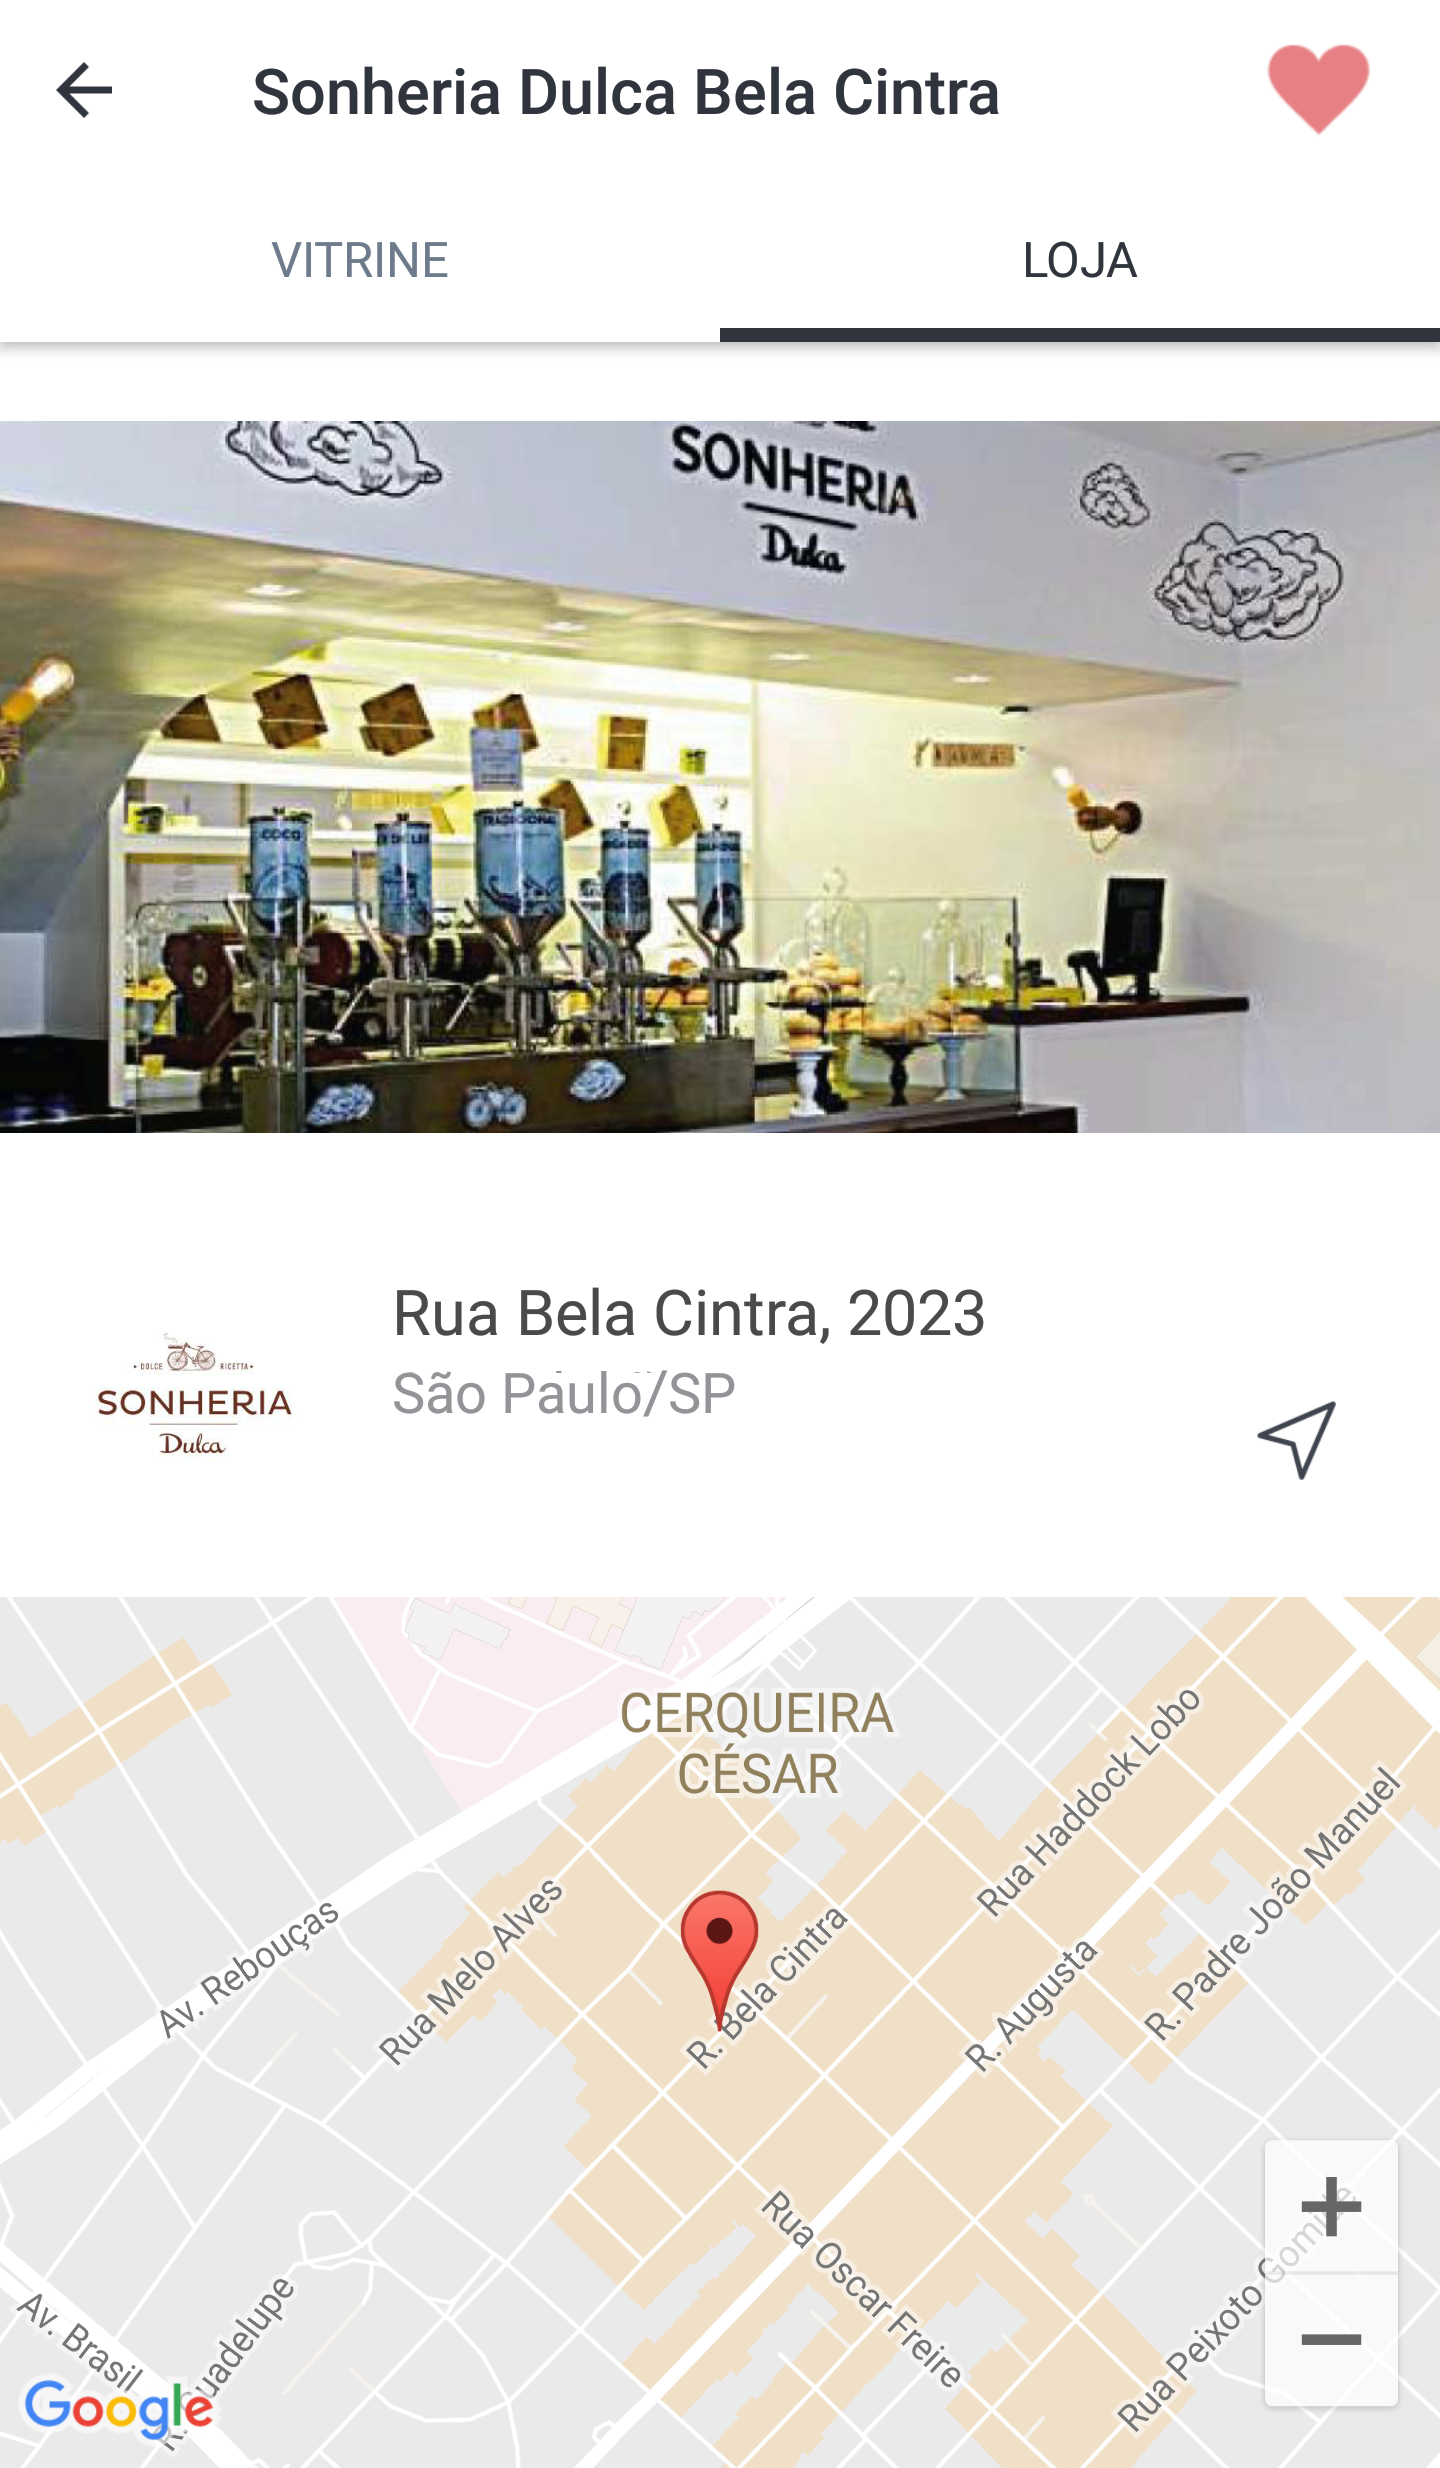
\includegraphics[scale=0.13]{img/info_parceiros}}
\label{fig:info_parceiros}
\caption* {Fonte: Aplicativo Beeconnect}
\end{figure}

\section{Testar Hipóteses}
\label{cha:testar_hipoteses}
Durante o mês de março a equipe focou em realizar os testes o mais rápido possível. 

\subsection{Teste da hipótese 1}
\label{cha:teste_1}
Para testar a hipótese 1 foi organizado um mutirão de vendas durante uma segunda-feira que focou na região da Paulista entre os metrôs Trianon-Masp e Consolação devido a proximidade com o escritório. Onze membros da Beeconnect participaram do mutirão organizados em cinco grupos, quatro duplas e um trio, cada grupo deveria percorrer uma das áreas, ilustradas na \autoref{fig:area_mutirao}.

\begin{figure}[H]
\caption{Área coberta pelo mutirão de vendas}
\centerline{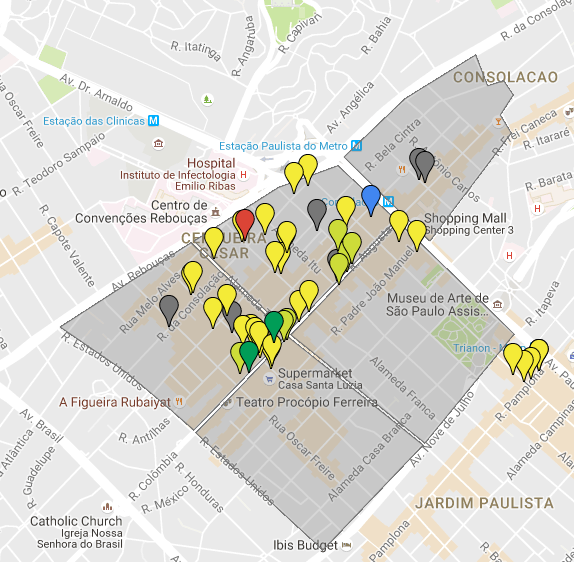
\includegraphics[scale=0.25]{img/area_mutirao}}
\label{fig:area_mutirao}
\caption* {Fonte: Elaborado pelo autor através da ferramenta do Google Maps}
\end{figure}

Durante o mutirão de vendas os membros da equipe tentaram vender primeiro o plano mensal com beacons que custava R\$99 por mês por beacon por loja, caso não houvesse interesse o membro oferecia o plano sem beacon que custava R\$49 por mês por loja. A equipe também carregava uma apresentação impressa, exemplo de slide na \autoref{fig:apresentacao_vendas_bc}, da Beeconnect para deixar com os funcionários da loja caso o dono não estivesse presente.

\begin{figure}[H]
\caption{Exemplo de slide da Apresentação de Vendas}
\centerline{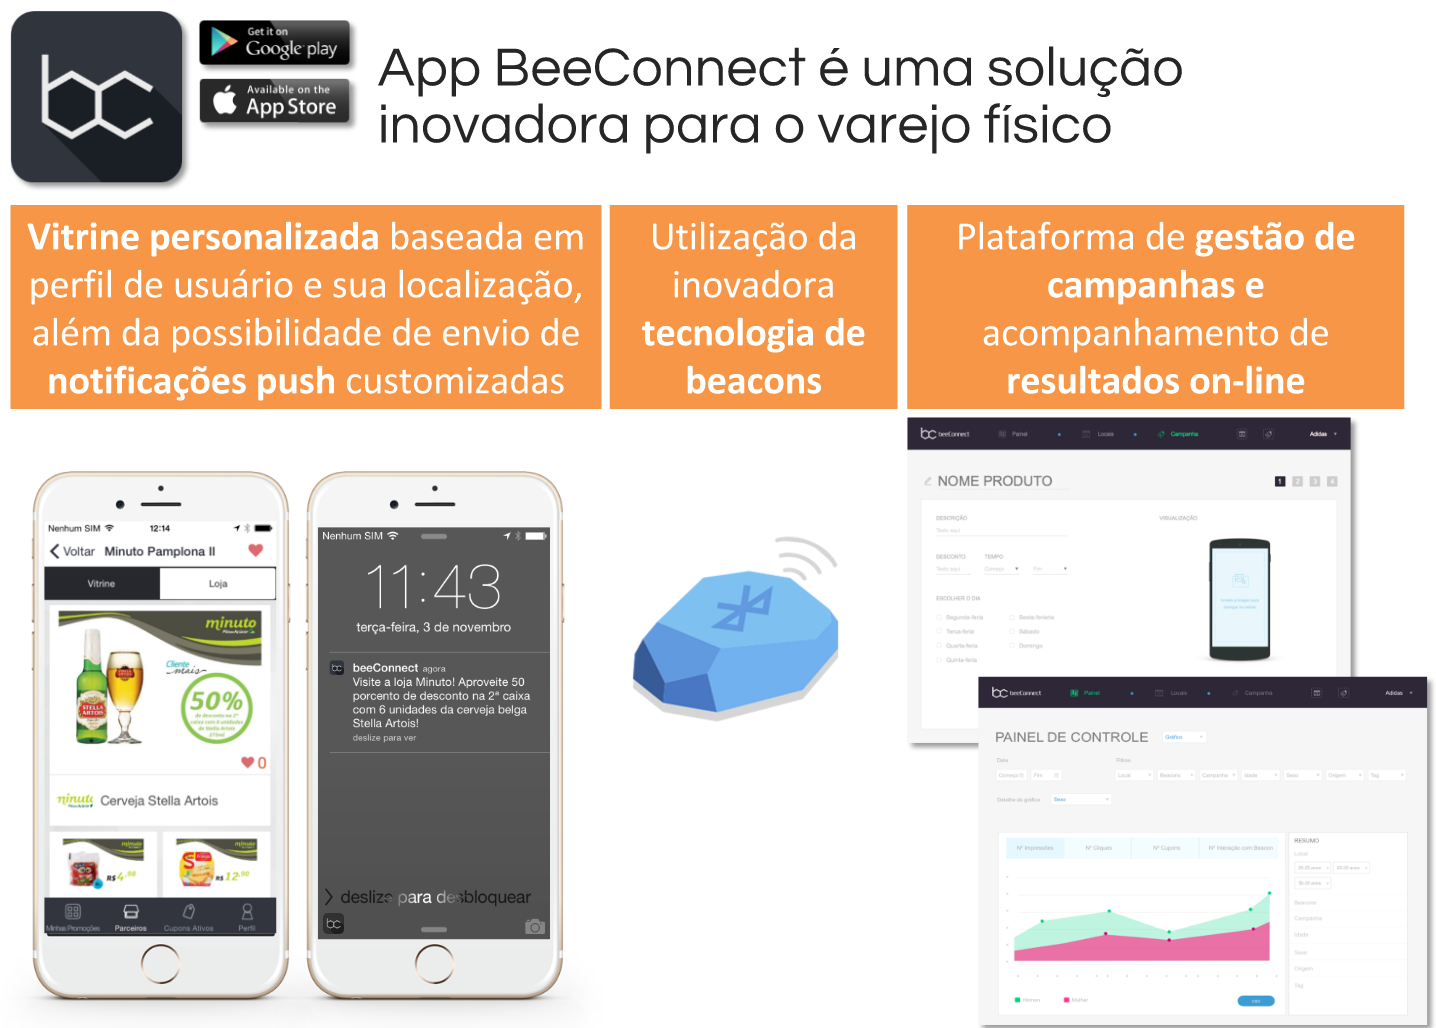
\includegraphics[width=0.8\textwidth]{img/apresentacao_vendas_bc}}
\label{fig:apresentacao_vendas_bc}
\caption* {Fonte: Material de vendas da Beeconnect}
\end{figure}

\subsection{Teste da hipótese 2}
\label{cha:teste_2}
Para o teste da hipótese 2, que foi realizado dois dias após o mutirão de vendas, o time comercial da startup ligou para todos os varejistas que estavam dentro do aplicativo para perguntar se eles estavam dispostos a dar pelo menos um desconto exclusivo no aplicativo.

\subsection{Teste da hipótese 3}
\label{cha:teste_3}
O teste da hipótese 3 foi realizado dois dias após a realização do teste 2, ou seja, em uma sexta-feira. A equipe da Beeconnect criou um post pago no Facebook, conforme mostra a \autoref{fig:post_sonheria}, com a melhor oferta disponível no aplicativo na época, "50\% de desconto na compra do segundo sonho" na Sonheria Dulca. Na campanha de marketing a equipe mirou no público que havia dado curtir na página do Facebook da Sonheria. A campanha rodou por 1 dia por motivos de orçamento.

\begin{figure}[H]
\caption{Post Facebook Sonheria Dulca}
\centerline{
\includegraphics[width=0.8\textwidth]{img/post_sonheria}}
\label{fig:post_sonheria}
\caption* {Fonte: Material de marketing da Beeconnect}
\end{figure}

\subsection{Teste da hipótese 4}
\label{cha:teste_4}
Para o teste da hipótese 4, que começou um dia após a realização do teste 3, utilizou-se do monitoramento desenvolvido dentro do aplicativo para analisar o comportamento dos usuários que baixaram o app através do post feito no Facebook. O objetivo era ver quantos usuários únicos iriam gerar cupom durante a primeira semana de experiência do aplicativo.

\subsection{Teste da hipótese 5}
\label{cha:teste_5}
Para testar a hipótese 5 foi realizado após uma semana em relação ao teste 4 com intuito de fazer uma análise de coorte do grupo de usuários que foi impactado pelo post feito no Facebook. Analisou-se quantos usuários que geraram cupom na semana anterior também geraram cupom naquela semana.

\subsection{Teste da hipótese 6}
\label{cha:teste_6}
O teste da hipótese 6 foi realizado em paralelo com os teste 4 e 5. Através do monitoramento feito no aplicativo foi possível analisar quantos usuários únicos acessaram a tela de informações da Sonheria Dulca, ilustrada na \autoref{fig:info_parceiros}.

\section{Analisar Resultados e Repetir Ciclo}
\label{cha:analisar_resultados}
Essa seção apresenta quais foram os resultados obtidos durante a fase de testes assim como faz uma análise desses resultados.

\subsection{Resultado do Teste da hipótese 1}
\label{cha:resultado_1}
Durante esse teste foram visitadas 70 lojas, sendo que 10 decidiram fazer parte do aplicativo, ou seja, pouco mais que 14\% das lojas foram convertidas, como mostra a \autoref{tab:resultado_1}. Dado que a porcentagem esperada de lojas convertidas era de 10\%, pode-se dizer que a Beeconnect passou no teste.
\begin{table}[H]
\centering
\caption{Resultado do teste da hipótese 1}
\label{tab:resultado_1}
\begin{tabular}{cccc}
Lojas Visitadas & Lojas Convertidas & Resultado & Esperado          \\
70                        & 10                          & 14.3\%      & \textgreater 10\%
\end{tabular}
\caption* {Fonte: Elaborado pelo autor}    
\end{table}

\subsection{Resultado do Teste da hipótese 2}
\label{cha:resultado_2}
Ao ligar para os varejistas, os vendedores da Beeconnect conseguiram que 12 das 28 lojas parceiras no momento disponibilizassem descontos exclusivos para o aplicativo, ou seja, pouco mais que 42\%, como mostra a \autoref{tab:resultado_2}. Nesse teste também pode-se concluir que a startup passou no teste dado que seu resultado de 42\% foi maior que o esperado de 40\%.
\begin{table}[H]
\centering
\caption{Resultado do teste da hipótese 2}
\label{tab:resultado_2}
\begin{tabular}{cccc}
Lojas com Desconto Exclusivo & Lojas Parceiras & Resultado & Esperado          \\
12                       & 28                          & 42.8\%      & \textgreater 40\%
\end{tabular}
\caption* {Fonte: Elaborado pelo autor}    
\end{table}

\subsection{Resultado do Teste da hipótese 3}
\label{cha:resultado_3}
O post no Facebook feito para a campanha da Sonheria rendeu 90 downloads do aplicativo, sendo visto por 55440 vezes, o que deu uma conversão de 0,23\%, que ficou bem abaixo do esperado de 1\%, referenciado na \autoref{tab:resultado_3_1}. Cada download custou cerca de R\$ 4,43, bem acima que o esperado de R\$1,00, como visto na \autoref{tab:resultado_3_2}. Portanto, os dois resultados do teste com o post no Facebook foram bem insatisfatórios para a Beeconnect.
\begin{table}[H]
\centering
\caption{Resultado 1 do teste da hipótese 3}
\label{tab:resultado_3_1}
\begin{tabular}{cccc}
Downloads & Alcance & Conversão & Conversão Esperada \\
90                       & 55440 &  0.23\%     & \textgreater 1\%
\end{tabular}
\caption* {Fonte: Elaborado pelo autor}    
\end{table}

\begin{table}[H]
\centering
\caption{Resultado 2 do teste da hipótese 3}
\label{tab:resultado_3_2}
\begin{tabular}{ccc}
Custo por Download & Custo por Download Esperado \\
R\$4,43          & \textless R\$1,00
\end{tabular}
\caption* {Fonte: Elaborado pelo autor}    
\end{table}


\subsection{Resultado do Teste da hipótese 4}
\label{cha:resultado_4}
Dos 90 usuários que baixaram o aplicativo através do Post do Facebook criado para a hipótese 3, 11 conseguiram gerar ao menos um cupom na primeira semana de uso do aplicativo, uma conversão de pouco mais que 12\%. Portanto, o resultado foi positivo para empresa dado que o esperado era que 10\% dos usuários gerassem cupons, como mostra a \autoref{tab:resultado_4}.
\begin{table}[H]
\centering
\caption{Resultado do teste da hipótese 4}
\label{tab:resultado_4}
\begin{tabular}{cccc}
Usuários & Usuários Únicos com Cupom & Conversão & Conversão Esperada \\
90       & 11  & 12.2\%   & \textgreater 10\%
\end{tabular}
\caption* {Fonte: Elaborado pelo autor}    
\end{table}

\subsection{Resultado do Teste da hipótese 5}
\label{cha:resultado_5}
Dos 11 usuários que geraram pelo menos um cupom na primeira semana de uso do aplicativo, 3 geraram pelo menos um cupom na segunda semana do aplicativo, pouco mais de 27\%, conforme mostra a \autoref{tab:resultado_5}. Como mencionado anteriormente, o resultado esperado era de 25\%, portanto a empresa teve um resultado positivo quanto a um teste de retenção.
\begin{table}[H]
\centering
\caption{Resultado do teste da hipótese 5}
\label{tab:resultado_5}
\begin{tabular}{cccc}
Usuários com cupom semana 1 & Usuários com cupom semana 2 & Resultado & Esperado \\
11       & 3  & 27.2\%   & \textgreater 25\%
\end{tabular}
\caption* {Fonte: Elaborado pelo autor}    
\end{table}

\subsection{Resultado do Teste da hipótese 6}
\label{cha:resultado_6}
Quanto ao teste de consultas à tela de informações do parceiro, dos 90 usuários que baixaram o aplicativo, 15 consultaram ao menos uma vez essa tela durante as duas semanas de monitoramento, cujo resultado dá aproximadamente 17\%, muito aquém dos 30\% esperados, como mostra a \autoref{tab:resultado_6}.
\begin{table}[H]
\centering
\caption{Resultado do teste da hipótese 6}
\label{tab:resultado_6}
\begin{tabular}{cccc}
Usuários & Usuários que consultaram a tela de informações & Resultado & Esperado \\
90       & 15  & 16.7\%   & \textgreater 30\%
\end{tabular}
\caption* {Fonte: Elaborado pelo autor}    
\end{table}

Dados os resultados dos testes o autor decidiu iterar pelo ciclo mais uma vez para aprender mais sobre o modelo de negócio da startup.

\section{Mapear estado atual da startup 2}
\label{cha:mapear_estado_2}
A partir da evolução na compreensão do modelo de negócio da Beeconnect a equipe decidiu elaborar um novo Canvas de Modelo Negócio, referenciado na \autoref{fig:canvas_beeconnect_2}, para que ficasse mais fácil de visualizar os novos aprendizados. Só foram feitos alguns ajustes em relação ao canvas inicial nos blocos:

\begin{itemize}
\item Proposta de Valor: somente houve um ajuste na formulação dos descontos exclusivos para "Cupons de descontos exclusivos".
\item Segmentos de Clientes: A modificação feita foi de "Compradores que gostam de descontos" para "Compradores de lojas físicas". O motivo dessa mudança foi porque o aplicativo não quer focar nos compradores de lojas virtuais, e também dado que o aplicativo também tem a função de ser um panfleto digital, aumentar o escopo para compradores de lojas físicas pode aumentar a base de usuários.
\item Fluxo de Receita: Dada as conversas com os próprios varejistas muitos perguntavam se o usuário teria que pagar alguma quantia para usufruir do aplicativo. A equipe decidiu deixar claro no canvas que o usuário não iria desembolsar nada para utilizar o app.
\end{itemize}

\begin{figure}[H]
\caption{Canvas de Modelo de Negócio após testes}
\centerline{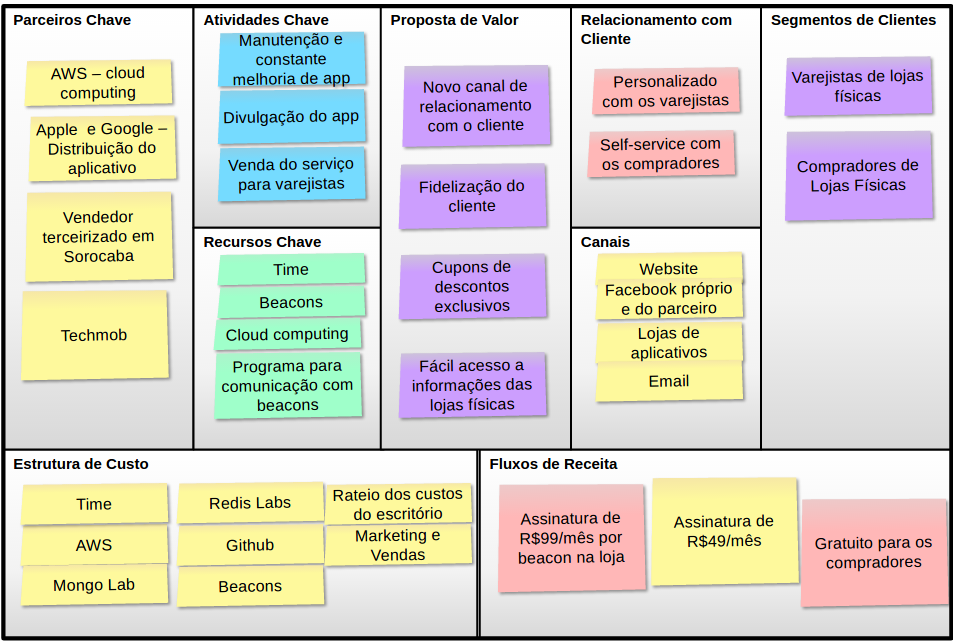
\includegraphics[width=0.8\textwidth]{img/canvas_beeconnect_2}}
\label{fig:canvas_beeconnect_2}
\caption* {Fonte: Elaborado pelo autor}
\end{figure}


\section{Listar Lições Aprendidas}
\label{cha:listar_licoes_aprendidas}